\documentclass[tikz,border=0pt]{standalone}
\usepackage{fontspec}
\setmainfont{DejaVu Serif}[Ligatures=NoCommon]
\definecolor{ink}{HTML}{252525}

% An open arrowhead, with dimensions in PDF points.
\newcommand{\flowarrow}[4]{%
  \draw[line width=.75bp, line cap=round, line join=round]
    (#1) -- (#2);
  \draw[line width=.75bp, line cap=round, line join=round]
    ([xshift=#3bp,yshift=#4bp]#2) -- (#2)
    -- ([xshift=-#3bp,yshift=#4bp]#2);
}

\begin{document}
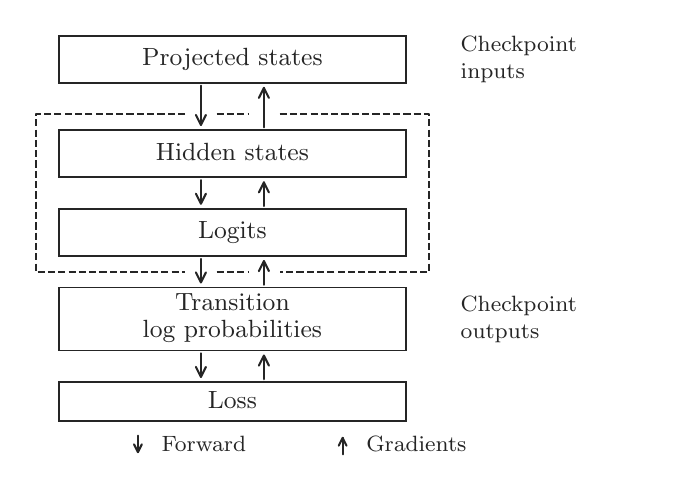
\begin{tikzpicture}[
  x=1mm, y=1mm, draw=ink, text=ink,
  font=\fontsize{9bp}{11bp}\selectfont,
  every node/.style={inner sep=0pt, outer sep=0pt},
  label/.style={anchor=base, yshift=-2.484375bp},
  small label/.style={anchor=base west, font=\fontsize{8bp}{10bp}\selectfont}]
  \path[use as bounding box] (0,0) rectangle (80,55);
  \begin{scope}[overlay]
    % The enclosure leaves a gap around each forward/gradient arrow.
    \draw[line width=.7bp, dash pattern=on 2.59bp off 1.12bp, line join=round]
      (20,44) -- (1,44) -- (1,24) -- (20,24);
    \draw[line width=.7bp, dash pattern=on 2.59bp off 1.12bp, line join=round]
      (32,44) -- (51,44) -- (51,24) -- (32,24);
    \foreach \y in {24,44}
      \draw[line width=.7bp, dash pattern=on 2.59bp off 1.12bp] (24,\y) -- (28,\y);

    \foreach \bottom/\height in {48/6,36/6,26/6,14/8,5/5}
      \draw[fill=white, line width=.7bp] (4,\bottom) rectangle ++(44,\height);
    \node[label,yshift=.0625bp] at (26,51) {Projected states};
    \node[small label,yshift=2.58359375bp] at (55,51) {Checkpoint};
    \node[small label,yshift=-6.98984375bp] at (55,51) {inputs};
    \node[label] at (26,39) {Hidden states};
    \node[label,yshift=.125bp] at (26,29) {Logits};
    \node[label] at (26,20) {Transition};
    \node[label,yshift=.0625bp] at (26,16.5) {log probabilities};
    \node[small label,yshift=2.58359375bp] at (55,18) {Checkpoint};
    \node[small label,yshift=-6.98984375bp] at (55,18) {outputs};
    \node[label] at (26,7.5) {Loss};

    % Values travel down; gradients with respect to the same tensors travel up.
    \foreach \upper/\lower in {48/42,36/32,26/22,14/10} {
      \coordinate (forwardstart) at ([yshift=-1bp]22,\upper);
      \coordinate (forwardend) at ([yshift=1.838525bp]22,\lower);
      \coordinate (gradientstart) at ([yshift=1bp]30,\lower);
      \coordinate (gradientend) at ([yshift=-1.838525bp]30,\upper);
      \flowarrow{forwardstart}{forwardend}{1.8}{3.6}
      \flowarrow{gradientstart}{gradientend}{1.8}{-3.6}
    }
    \coordinate (forwardstart) at (14,3.2);
    \coordinate (forwardend) at ([yshift=.838525bp]14,.8);
    \flowarrow{forwardstart}{forwardend}{1.4}{2.8}
    \coordinate (gradientstart) at (40,.8);
    \coordinate (gradientend) at ([yshift=-.838525bp]40,3.2);
    \flowarrow{gradientstart}{gradientend}{1.4}{-2.8}
    \node[small label,yshift=-2.203125bp] at (17,2) {Forward};
    \node[small label,yshift=-2.203125bp] at (43,2) {Gradients};
  \end{scope}
\end{tikzpicture}
\end{document}
